\subsection{Stability}
\label{subsec:stability}

Stability, when referring to a clock source, is the measure of how well the reference frequency can be maintained over time.
All the metrics used to define the stability of a clock are based on the fractional frequency error, which is the ratio between the frequency error and the reference frequency, namely:

\begin{equation}
  y(t) = \frac{f(t) - f_0}{f_0}
  \label{eq:fractional_frequency_error}
\end{equation}

Where $f(t)$ is the frequency of the clock at time $t$, and $f_0$ is the nominal frequency of the clock.

In the framework of \acrshort{csacs}, or more in general of atomic clocks, three main regions can be identified in the stability plot: short-term, medium-term, and long-term stability.

\begin{figure}[H]
  \centering
  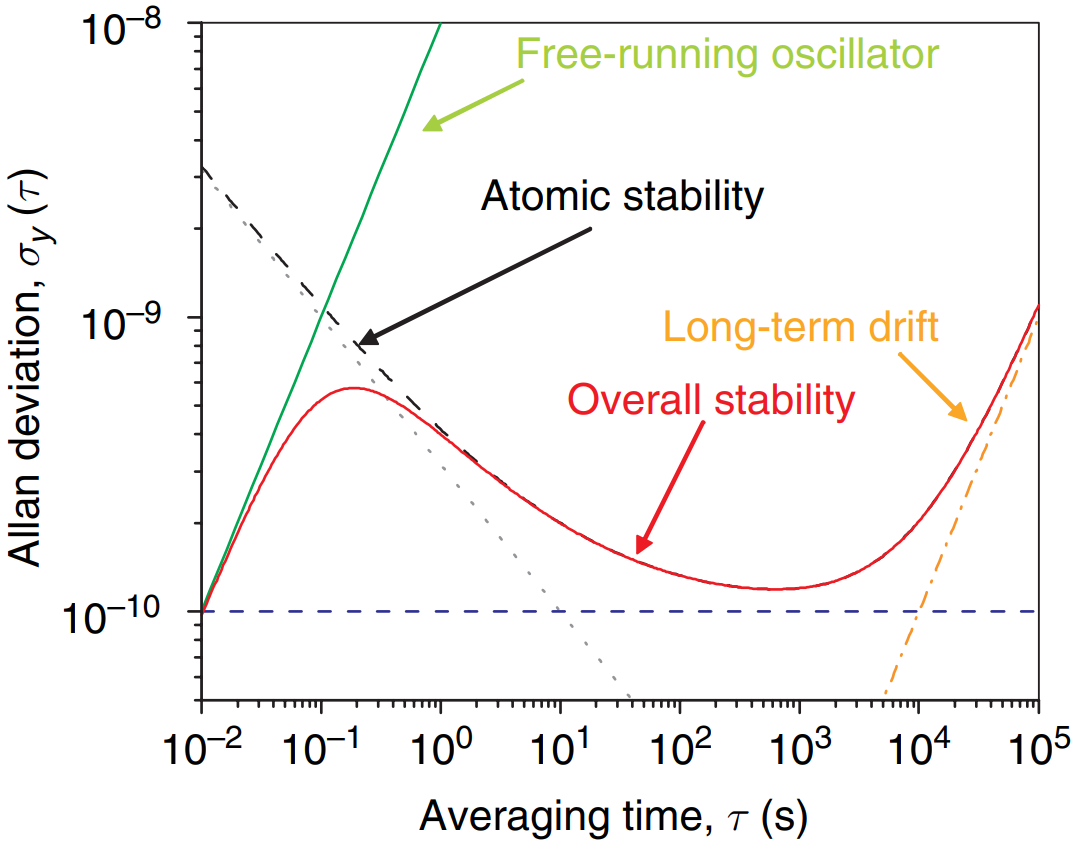
\includegraphics[width=0.6\textwidth, max width=\linewidth]{img/overall-statbility-contributions.png}
  \caption{
    Overall stability of a clock source as summation of the different contributions from the internal components and processes.
    Observing the overall stability (red line), we can distinguish three main regions: short-term ($0 \le \tau \le 10^{0}s$), medium-term ($10^0 \le \tau \le 10^{3}s$), and long-term (beyond the flicker floor).
    Source \cite{Knappe}.
  }
  \label{fig:overall-statbility-contributions}
\end{figure}

\subsubsection{Short-term stability}

Short-term stability refers to the performance of a clock over very short time intervals, typically ranging from a few milliseconds to a few seconds.
Allan deviation (denoted as $\sigma_y(\tau)$) is the metric used to measure it, capturing both rapid fluctuations (Fast Noise) and gradual drifts (Slow Drift) in the output frequency.
From its definition, Allan deviation (ADEV) can be computed as:

\begin{equation}
  \sigma_y(\tau) = \sqrt{\frac{1}{2M} \sum_{i=2}^{M} (\bar{y}(\tau)_{i} - \bar{y}(\tau)_{i-1})^2}
  \label{eq:allan_deviation_short}
\end{equation}

Where $\bar{y}(\tau)_{i}$ is the average fractional frequency error over the time interval $\tau$ and $M$ is the number of sampling data.

To give a more practical example, we can consider a clock running with an output frequency of $f_0 = 10MHz$, having an Allan deviation of $\sigma_y(\tau=1s) = 3 \times 10^{-9}$.
In this case, the instability in frequency between two observations 1 second apart has an RMS value of $3 \times 10^{-9}$, that means a $10MHz * 3 \times 10^{-9} = 30mHz$ RMS\footnote{RMS: Room Mean Square} movement in frequency mostly due to the Fast Noise.

As we will see in Section \ref{sec:performances_and_limitations}, for a \acrshort{csac} clock the component having a major impact on the Fast Noise is the \acrfull{lo}.


\subsubsection{Medium-term stability}

Medium-term stability refers to the performance of a clock over longer time intervals, typically ranging from a few seconds to a few minutes or hours.
Allan deviation is again the metric used to measure it.
In this case however, ADEV can be computed using an approximated version of Equation \ref{eq:allan_deviation_short}:

\begin{equation}
  \sigma_y(\tau) = \frac{1}{Q \times SNR} \tau^{-1/2}
  \label{eq:allan_deviation_medium}
\end{equation}

Where $Q = \frac{\nu_0}{\Delta \nu}$ and $SNR = \frac{P_{signal}}{P_{noise}}$ are related to the quality of the output signal in terms of frequency and power.

This simplified version of the Allan deviation can be adopted knowing that Fast Noise is no longer the main source of instability, and the Slow Drift becomes the dominant factor.

As we will see in Section \ref{sec:performances_and_limitations}, for a \acrshort{csacs} clock, the cause of the medium-term stability cannot be brought back to a single component, but it's the result of multiple and concurrent effects.

\subsubsection{Long-term stability}

Long-term stability refers to the performance of a clock over very long time intervals, typically ranging from a few days to a few years.
Fractional frequency error is the metric used to measure this, and it's computed from the definition given in Equation \ref{eq:fractional_frequency_error}.

It's common to consider as the starting point from which consider long-term stability region, the flicker floor.
On a $\sigma_y(\tau)$ plot, the flicker floor can be identified as the point where the Allan deviation reaches a minimum value and then starts to increase again.

At such long time scale, multiple factors influence this metric as for example aging, environmental conditions, and other external factors.
The summation of all these factors is usually referred to as Drift.

